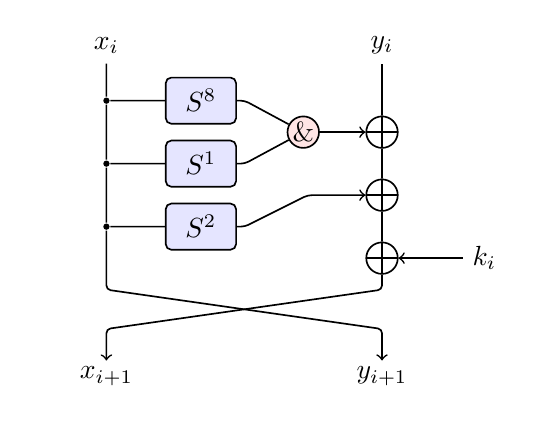
\begin{tikzpicture}
  [line width=0.6,trim left,
   shiftbox/.style = {
     draw, fill=blue!10, rounded corners=2pt,
     inner xsep=0.25cm, inner ysep=0.15cm,
   },
   wire/.style = {
     rounded corners=1.5pt
   },
   xor/.style = {
     draw, circle, inner sep=0cm, minimum size=0.4cm,
     append after command = {
       [shorten >=\pgflinewidth, shorten <=\pgflinewidth,]
       (\tikzlastnode.north) edge (\tikzlastnode.south)
       (\tikzlastnode.east) edge (\tikzlastnode.west)
     }
   },
   odot/.style = {
     draw, circle, inner sep=0cm, minimum size=0.4cm,fill=red!10
   },
   dot/.style = {
     fill, circle, inner sep=0cm, minimum size=0.08cm
   }]

  %Draw nodes
  \node at (1,6.7) (xin) {$x_i$};
  \node at (4.5,6.7) (yin) {$y_i$};
  \node[dot] at (1,6) (d1) {};
  \node[dot] at (1,5.2) (d2) {};
  \node[dot] at (1,4.4) (d3) {};
  \node[shiftbox] at (2.2,6) (S1) {$S^8$};
  \node[shiftbox] at (2.2,5.2) (S2) {$S^1$};
  \node[shiftbox] at (2.2,4.4) (S3) {$S^2$};
  \node[xor] at (4.5,5.6) (x1) {};
  \node[xor] at (4.5,4.8) (x2) {};
  \node[xor] at (4.5,4.0) (x3) {};
  \node[odot] at (3.5,5.6) (AND) {\&};
  \node at (5.8,4.0) (k) {$k_i$};
  \node at (1, 2.5) () {$x_{i+1}$};
  \node at (4.5, 2.5) () {$y_{i+1}$};

  %Draw wires
  \draw[wire] (d1) -- (S1)  (S1.east) -- +(0.1,0) -- (AND);
  \draw[wire] (d2) -- (S2)  (S2.east) -- +(0.1,0) -- (AND);
  \draw[wire,->] (AND) -- (x1);
  \draw[wire,->] (d3) -- (S3) (S3.east) -- +(0.1,0) -- ++(0.9,0.4) -- (x2);
  \draw[wire,->] (xin) -- (d1) -- (d2) -- (d3)
                  -- ++(0,-0.8) -- ++(3.5,-0.5) -- ++(0,-0.4);
  \draw[wire,->] (yin) -- (x1) -- (x2) -- (x3)
                 -- ++(0,-0.4) -- ++(-3.5,-0.5) -- ++(0,-0.4);
  \draw[wire,->] (k.west) -- (x3);
\end{tikzpicture} 